\section{Ziele des Versuchs}
In diesem Versuch sollen anhand des Quadrupol-Massenspektrometers (QMS) die Methoden der Massenspektrometrie und die Grundlagen der Vakuum-Physik vermittelt werden. Die Massenspektrometrie ist ein wichtiges Analyseverfahren, um die Struktur und die Zusammensetzung verschiedener chemischer Elemente und Gemische zu analysieren.\\

\section{Theoretische Grundlagen}
\subsection{Der Quadrupol-Massenspektrometer}
Ein Quadrupol-Massenspektrometer erzeugt ein statisches elektrisches Feld. Je nach Stärke des Feldes und dem Ladungs-/Massenverhältnis der Ionen, bewegen sich diese auf stabilen oder instabilen Bahnen. Abhängig davon wie die Spannung variiert wird, gelangen Ionen verschiedener Ladungs/-Massenverhältnisse auf stabile Bahnen und auf diesen durch den QMS. Diesen Filtervorgang nennt man Massenfiltern.\\
Das Quadrupol-Massenspektrometer befindet sich dabei in einer Vakuum-Kammer (Rezipient), um ungewollte Stöße der Ionen mit anderen Teilchen zu vermeiden und um zu gewährleisten, dass die Ionen auch wirklich den Detektor erreichen. Dieses Vakuum wird mit zwei Pumpen erzeugt (siehe Abb. 1). Der Detektor misst den Ionenstrom und sendet die Daten an einen Computer. Mit Hilfe eine Software (in unserem Fall ein LabView-Programm) werden anschließend die Daten ausgewertet.

\myImage[13cm]{img/qme1}{Quadrupolmassenspektrometer (a) Äquipotentiallinien; (b) hyperbolische Elektroden [3]}

\newpage
\subsection{Die Mathieuschen Differentialgleichung}
Die jeweils gegenüberliegenden Stäbe werden elektrisch miteinander verbunden und paarweise an den positiven bzw. negativen Pol einer variablen Spannungsquelle angeschlossen. Zudem werden Wechselspannungsfelder ($f \approx 10^8$ Hz) mit einer Phasendifferenz zwischen den Stabpaaren von $\phi = 180^{\circ}$ überlagert.
Wolfgang Paul beschrieb das Potential eines Quadrupols in kartesischen Koordinaten durch folgende Gleichung [1]:

\begin{equation}
\mathbf{\Phi} = \frac{\Phi_{0}}{2r^{2}}\left(\alpha x^{2}+\beta y^{2}+\gamma z^{2}\right)
\end{equation}

Durch Anwendung der Laplace'schen Differentialgleichung $\Delta \mathbf{\Phi} =0$ ergibt sich für die Koeffizienten die Bedingung:

\begin{equation}
\Delta \mathbf{\Phi} = \alpha + \beta +\gamma =0
\end{equation}

mit je einer Lösung für ein zweidimensionales und ein dreidimensionales Feld.\\
Wir betrachten nun die zweidimensionale Lösung. Es gilt $\alpha = -\gamma = 1$, $\beta =0$. Daraus folgt:

\begin{equation}
\mathbf{\Phi} = \frac{\Phi_{0}}{2r_{0}^{2}}\left(x^{2}-z^{2}\right)
\end{equation}

Diese Bedingungen werden durch ein elektrisches Feld erfüllt, welches durch vier hyperbolisch geformte Stabelektroden induziert wird (siehe Abb. 1). Das Koordinatensystem definiert man anschließend so, dass die y-Achse parallel zu den Elektroden verläuft.
\\
Die elektrische Feldstärke $\mathbf{E}$ errechnet sich aus der Gleichung $-\mathbf{\triangledown \Phi} = \mathbf{E}$. Daraus folgt für $\mathbf{E}$ mit den oben genannten Bedingungen:

\begin{equation}
-\mathbf{\triangledown \Phi} = \mathbf{E} =
\left(
\begin{matrix}
-\Phi_{0}/r_{0}^{2} \cdot x\\
0\\
\Phi_{0}/r_{0}^{2} \cdot z
\end{matrix}
\right)
\end{equation}

Die $E_x$-Komponente bewirkt, dass die Ionen eine sinusförmige Schwingung in der x-y-Ebene ausführen. Die $E_z$-Komponente bewirkt jedoch, dass das Ion exponentiell beschleunigt wird. Um dem entgegen zu wirken, wird ein Potential $\Phi_0$ benutzt, welches sich aus einer Gleich- und einer Wechselspannung zusammensetzt: 

\begin{equation}
\Phi_{0}=U + V cos(\omega t)
\end{equation}
\newpage
und für die Bewegungsgleichungen folgt daraus:

\begin{equation}
\ddot{x} + \frac{e}{mr_{0}^{2}}(U+V cos (\omega t)) x = 0
$$\\$$
\ddot{z} - \frac{e}{mr_{0}^{2}}(U+V cos (\omega t)) z = 0
\end{equation}

Das Feld im QMS (siehe Abb. 1 a)) ist ein periodisches inhomogenes Feld, weswegen sich die zeitabhängigen Terme nicht wegkürzen. Die Gleichungen aus (6) haben die Form von Mathieuschen Differentialgleichungen, deren Normalformen lauten:

\begin{equation}
\frac{d^{2}x}{t\tau^{2}}+(a_{x}+2q_{x}cos (2\tau)) x = 0
$$\\$$
\frac{d^{2}z}{t\tau^{2}}-(a_{z}+2q_{z}cos (2\tau)) z = 0
\end{equation}

Aus dem Vergleich mit den Gleichungen (6) folgt, dass für die Parameter $a_{x}$, $a_{z}$, $q_{x}$, $q_{z}$ und $\tau$ folgendes gelten muss:

\begin{equation}
a_{x} = -a_{z} = \frac{4eU}{mr_{0}^{2}\omega^{2}},\qquad q_{x}= -q_{z}= \frac{4eV}{mr_{0}^{2}\omega^{2}} := b,\qquad \tau =\frac{\omega t}{2}
\end{equation}

Die Differentialgleichungen haben somit zwei Arten von Lösungen. Bei der einen Lösung bewegen sich die Ionen auf stabilen Bahnen. Sie oszillieren in x-z-Richtung und gelangen durch den Quadrupolfilter ohne die Elektroden zu berühren. Bei der zweiten Lösung vergrößert sich die Amplitude der Ionen in x-z-Richtung exponentiell. Dadurch bewegen sich die Ionen auf instabilen Bahnen und kollidieren mit den Elektroden (siehe Abb. 2 und 3)

\vspace{1cm}

\begin{figure}[h]
\centering
\begin{subfigure}{0.4\textwidth}
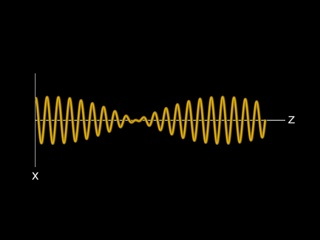
\includegraphics[width=\textwidth]{img/xzs}
\end{subfigure}
\begin{subfigure}{0.4\textwidth}
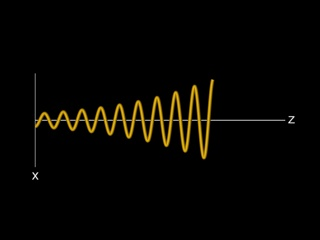
\includegraphics[width=\textwidth]{img/xzi}
\end{subfigure} 
\caption{Beispiel für eine stabile (links) und instabile Bahn (rechts)}
\end{figure}

\subsection{Stabilitätsdiagramme}
Um die Bewegung der Ionen durch den Quadrupol mathematisch-physikalisch zu beschreiben, benutzt man einen Graphen, in dem man q über a aufträgt (siehe Abb. 3, q entspricht hier b). Das Verhältnis $\frac{a}{q}=\frac{2U}{V}$ hängt nicht von der Masse der Ionen ab. Somit liegen alle Ionen verschiedener Massen im Stabilitätsdiagramm auf einer Geraden die durch den Nullpunkt geht. Variiert man U und V, so verändert man die Steigung der Arbeitsgeraden. Alle a/q-Werte, die stabile Flugbahnen durch den Quadrupol ergeben, liegen in Abb. 3 innerhalb des eingefärbten Feldes. Wird das Verhältnis von $\frac{U}{V}$ erhöht, wird die Steigung der Arbeitsgeraden größer und umso keiner wird das q-Intervall ($\Delta b$ in Abb. 3), bis nur noch Ionen einer bestimmten Masse auf stabilen Bahnen durch den Massenfilter zum Detektor gelangen.

\vspace{1cm}

\begin{figure}[h]
\centering
\begin{subfigure}{0.40\textwidth}
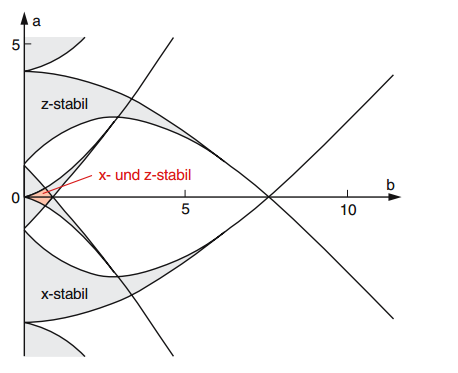
\includegraphics[width=\textwidth]{img/stab}
\end{subfigure}
\begin{subfigure}{0.40\textwidth}
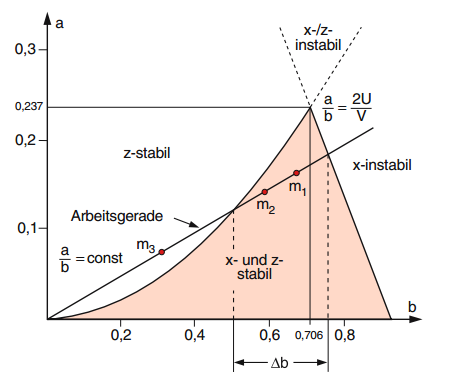
\includegraphics[width=\textwidth]{img/qme2}
\end{subfigure}
\caption{Stabilitätsdiagramme} 
\end{figure}

Um die Massen zu unterscheiden, definiert man die sogenannte Massenauflösung mit der Formel:
\begin{equation}
M = \frac{m}{\Delta m}
\end{equation} 

wobei $\Delta m$ die kleinste auflösbare Massendifferenz ist.

\section{Versuchsaufbau}
Das QMS muss während des Versuchs in einer Vakuum-Kammer sein. Das Vakuum wird durch eine Membran- und einer Turbomolekularpumpe erzeugt. Die Werte für den Druck liefert ein Druck-Messgerät, welches im Rezipienten ist. Die Testgase können über ein Feinriegelventil in den Rezipienten eingelassen werden. In der folgenden Skizze ist der Aufbau schematisch dargestellt:

\myImage[6cm]{img/aufbau}{Experimenteller Aufbau [3]}